%%%%%%%%%%%%%%%%%%%%%%%%%%%%%%%%%%%%%%%%%
% Jacobs Landscape Poster
% LaTeX Template
% Version 1.1 (14/06/14)
%
% Created by:
% Computational Physics and Biophysics Group, Jacobs University
% https://teamwork.jacobs-university.de:8443/confluence/display/CoPandBiG/LaTeX+Poster
% 
% Further modified by:
% Nathaniel Johnston (nathaniel@njohnston.ca)
%
% This template has been downloaded from:
% http://www.LaTeXTemplates.com
%
% License:
% CC BY-NC-SA 3.0 (http://creativecommons.org/licenses/by-nc-sa/3.0/)
%
%%%%%%%%%%%%%%%%%%%%%%%%%%%%%%%%%%%%%%%%%

%----------------------------------------------------------------------------------------
%	PACKAGES AND OTHER DOCUMENT CONFIGURATIONS
%----------------------------------------------------------------------------------------

\documentclass[final]{beamer}

\usepackage[scale=1.10]{beamerposter} % Use the beamerposter package for laying out the poster

\usetheme{confposter} % Use the confposter theme supplied with this template

\setbeamercolor{block title}{fg=nblue,bg=white} % Colors of the block titles
\setbeamercolor{block body}{fg=black,bg=white} % Colors of the body of blocks
\setbeamercolor{block alerted title}{fg=white,bg=dblue!70} % Colors of the highlighted block titles
\setbeamercolor{block alerted body}{fg=black,bg=dblue!10} % Colors of the body of highlighted blocks
% Many more colors are available for use in beamerthemeconfposter.sty

%-----------------------------------------------------------
% Define the column widths and overall poster size
% To set effective sepwid, onecolwid and twocolwid values, first choose how many columns you want and how much separation you want between columns
% In this template, the separation width chosen is 0.024 of the paper width and a 4-column layout
% onecolwid should therefore be (1-(# of columns+1)*sepwid)/# of columns e.g. (1-(4+1)*0.024)/4 = 0.22
% Set twocolwid to be (2*onecolwid)+sepwid = 0.464
% Set threecolwid to be (3*onecolwid)+2*sepwid = 0.708

\newlength{\sepwid}
\newlength{\onecolwid}
\newlength{\twocolwid}
\newlength{\threecolwid}
\setlength{\paperwidth}{48in} % A0 width: 46.8in
\setlength{\paperheight}{36in} % A0 height: 33.1in
\setlength{\sepwid}{0.024\paperwidth} % Separation width (white space) between columns
\setlength{\onecolwid}{0.22\paperwidth} % Width of one column
\setlength{\twocolwid}{0.464\paperwidth} % Width of two columns
\setlength{\threecolwid}{0.708\paperwidth} % Width of three columns
\setlength{\topmargin}{-0.5in} % Reduce the top margin size
%-----------------------------------------------------------

%My commands
\newcommand{\vp}{v_p}
\newcommand{\vs}{v_s}

\usepackage{amsmath}

\usepackage{graphicx}  % Required for including images

\usepackage{booktabs} % Top and bottom rules for tables


%----------------------------------------------------------------------------------------
%	TITLE SECTION 
%----------------------------------------------------------------------------------------

\title{Reconciling geophysical and geochemical constraints on the temperature and composition of cratonic lithosphere by considering mantle discontinuities} % Poster title

\author{Nicholas J. Mancinelli, Colleen A. Dalton, and Karen M. Fischer} % Author(s)

\institute{Department of Earth, Environmental, and Planetary Sciences; Brown University} % Institution(s)

%----------------------------------------------------------------------------------------

\begin{document}

\addtobeamertemplate{block end}{}{\vspace*{2ex}} % White space under blocks
\addtobeamertemplate{block alerted end}{}{\vspace*{2ex}} % White space under highlighted (alert) blocks

\setlength{\belowcaptionskip}{2ex} % White space under figures
\setlength\belowdisplayshortskip{2ex} % White space under equations

\begin{frame}[t] % The whole poster is enclosed in one beamer frame

\begin{columns}[t] % The whole poster consists of three major columns, the second of which is split into two columns twice - the [t] option aligns each column's content to the top

\begin{column}{\sepwid}\end{column} % Empty spacer column

\begin{column}{\onecolwid} % The first column

%----------------------------------------------------------------------------------------
%	OBJECTIVES
%----------------------------------------------------------------------------------------

\begin{alertblock}{Key Points}
\begin{itemize}
\item Key point A
\item Key point B
\item Key point C

\end{itemize}
\end{alertblock}

%----------------------------------------------------------------------------------------
%	INTRODUCTION
%----------------------------------------------------------------------------------------

\begin{block}{Geological Motivation}

Much of Earth's cratonic lithosphere has resisted deformation throughout geologic time.  Cooler-than-average temperatures make cratonic lithosphere strong and thick, and its depleted composition provides a buoyancy force which resists entrainment in deeper mantle flow.

\begin{itemize}

\item Surface-wave dispersion measurements place constraints on the absolute velocities of the cratonic mantle lithosphere, but it is difficult to reconcile these geophysical observations with the steady-state geotherms inferred from mantle xenoliths if a simple peridotite composition is assumed.
 
\item Xenolith-derived geotherms predict shear velocities that are higher than observed in the shallow mantle lithosphere and slower than observed in the deeper cratonic lithosphere.  One possible explanation is that a low-velocity layer pervades the shallow cratonic lithosphere, potentially a relict of metasomatic activity.

\item Scattered body-waves have suggested the presence of a negative velocity discontinuity at depths ranging from 90 to 140 km; these have been interpreted as the top of such a low-velocity zone.  At greater depths, converted waves occasionally reveal a velocity increase at a depth of $220\pm20$ km, the so-called Lehmann discontinuity, which is detected more often beneath continents than beneath oceans.

\end{itemize}

Here we plan to present an integrative perspective on cratonic temperature and composition by jointly analyzing surface wave observations (both shear velocity and attenuation), receiver functions (both Ps and Sp), and underside reflected waves (SS precursors) across the North American continent.

\end{block}

%------------------------------------------------

%\begin{figure}
%
\includegraphics[width=0.8\linewidth]{placeholder.jpg}
%\caption{Isochrons Figure.}
%\end{figure}

%----------------------------------------------------------------------------------------

\end{column} % End of the first column

\begin{column}{\sepwid}\end{column} % Empty spacer column

\begin{column}{\twocolwid} % Begin a column which is two columns wide (column 2)

\begin{columns}[t,totalwidth=\twocolwid] % Split up the two columns wide column

\begin{column}{\onecolwid}\vspace{-.6in} % The first column within column 2 (column 2.1)

%----------------------------------------------------------------------------------------
%	XENOLITH THERMOBAROMETRY
%----------------------------------------------------------------------------------------

\begin{block}{Geotherm Constraints from Xenoliths}

\begin{itemize}

\item Pressure--temperature constraints from xenoliths (cite CT Lee) and heat-flow modeling (cite Rudnick) to constrain a mantle geotherm.

\item Discuss assumptions

\begin{figure}
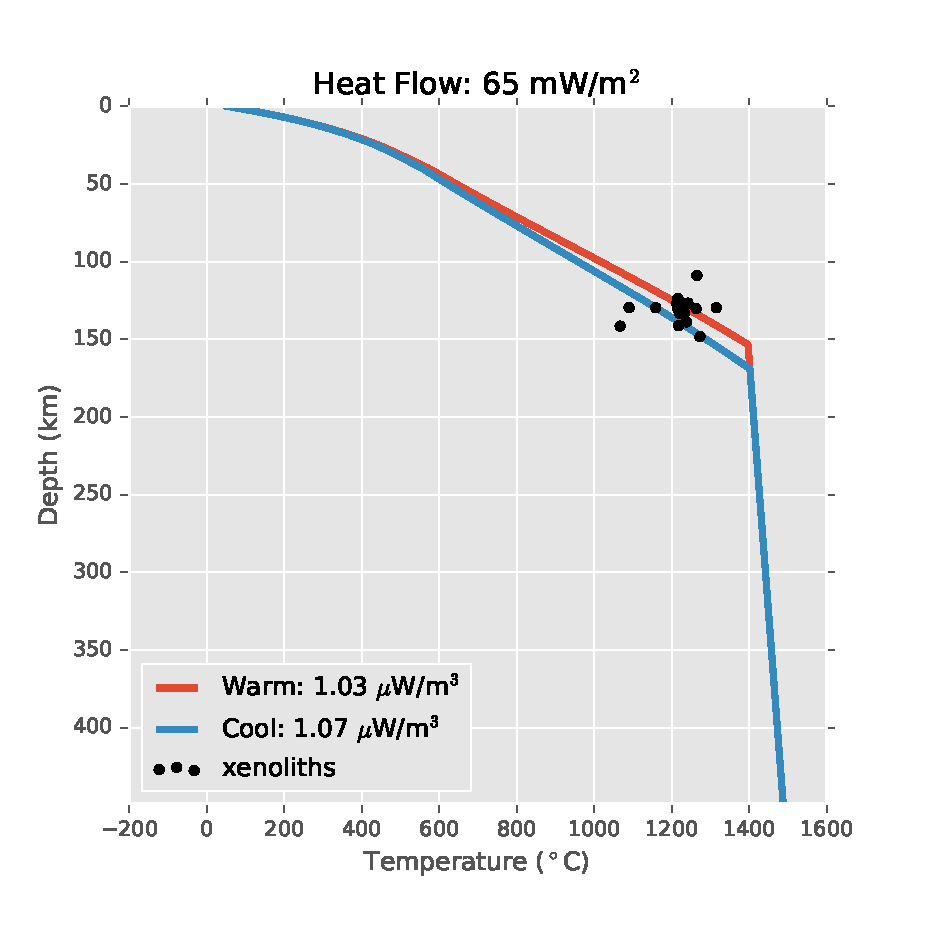
\includegraphics[width=0.5\textwidth]{img2/ColoradoPlateau_geotherm.eps}
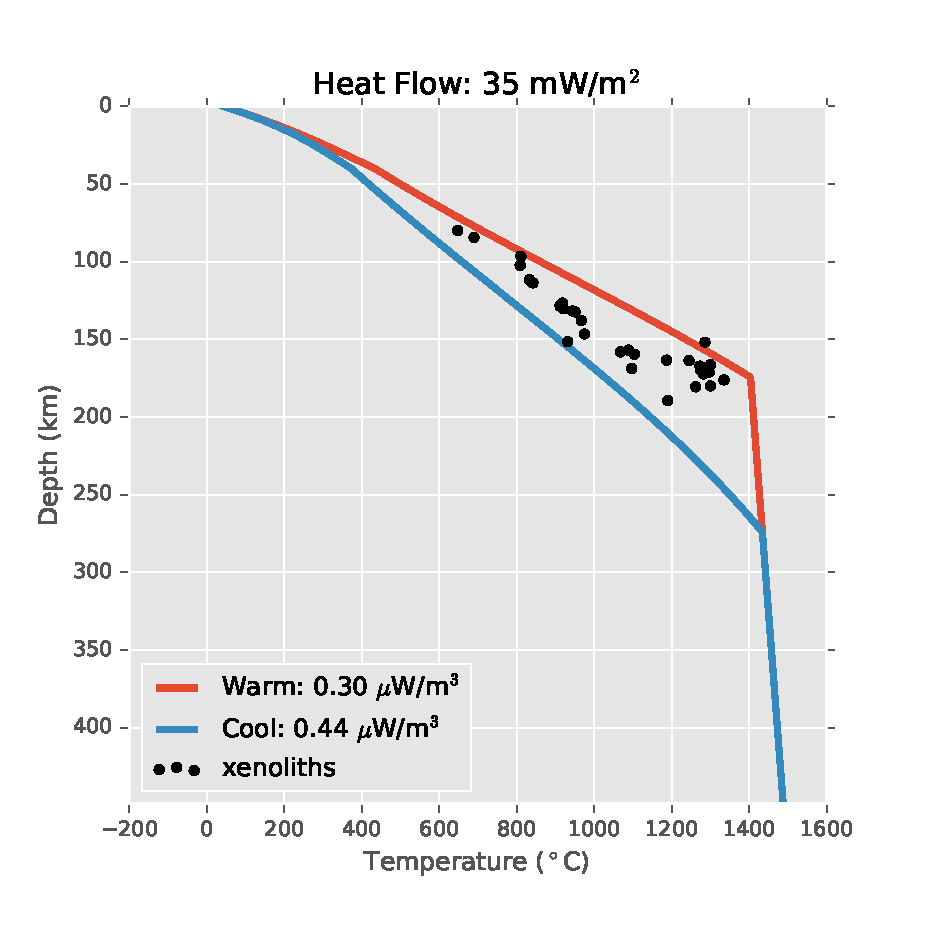
\includegraphics[width=0.5\textwidth]{img2/SlaveCraton_geotherm.eps}
\caption{Constraints on geotherms from xenolith thermobarometry.}
\end{figure}

\item Strong tradeoff between crustal heat production and surface heat-flow.  Solved by pegging heat-flow to defensible value, allow heat production to vary to match variability in the xenoliths.

\end{itemize}

\end{block}

%----------------------------------------------------------------------------------------

\end{column} % End of column 2.1

\begin{column}{\onecolwid}\vspace{-.6in} % The second column within column 2 (column 2.2)

%----------------------------------------------------------------------------------------
% PERPLEX CALCUOATIONS
%----------------------------------------------------------------------------------------

\begin{block}{Velocity Profiles from Mineral Physics}

\begin{itemize}

\item We used PerpleX (cite Connolly) to compute densities and seismic velocities for fertile and depleted compositions down to a depth of 350 km.

\begin{figure}
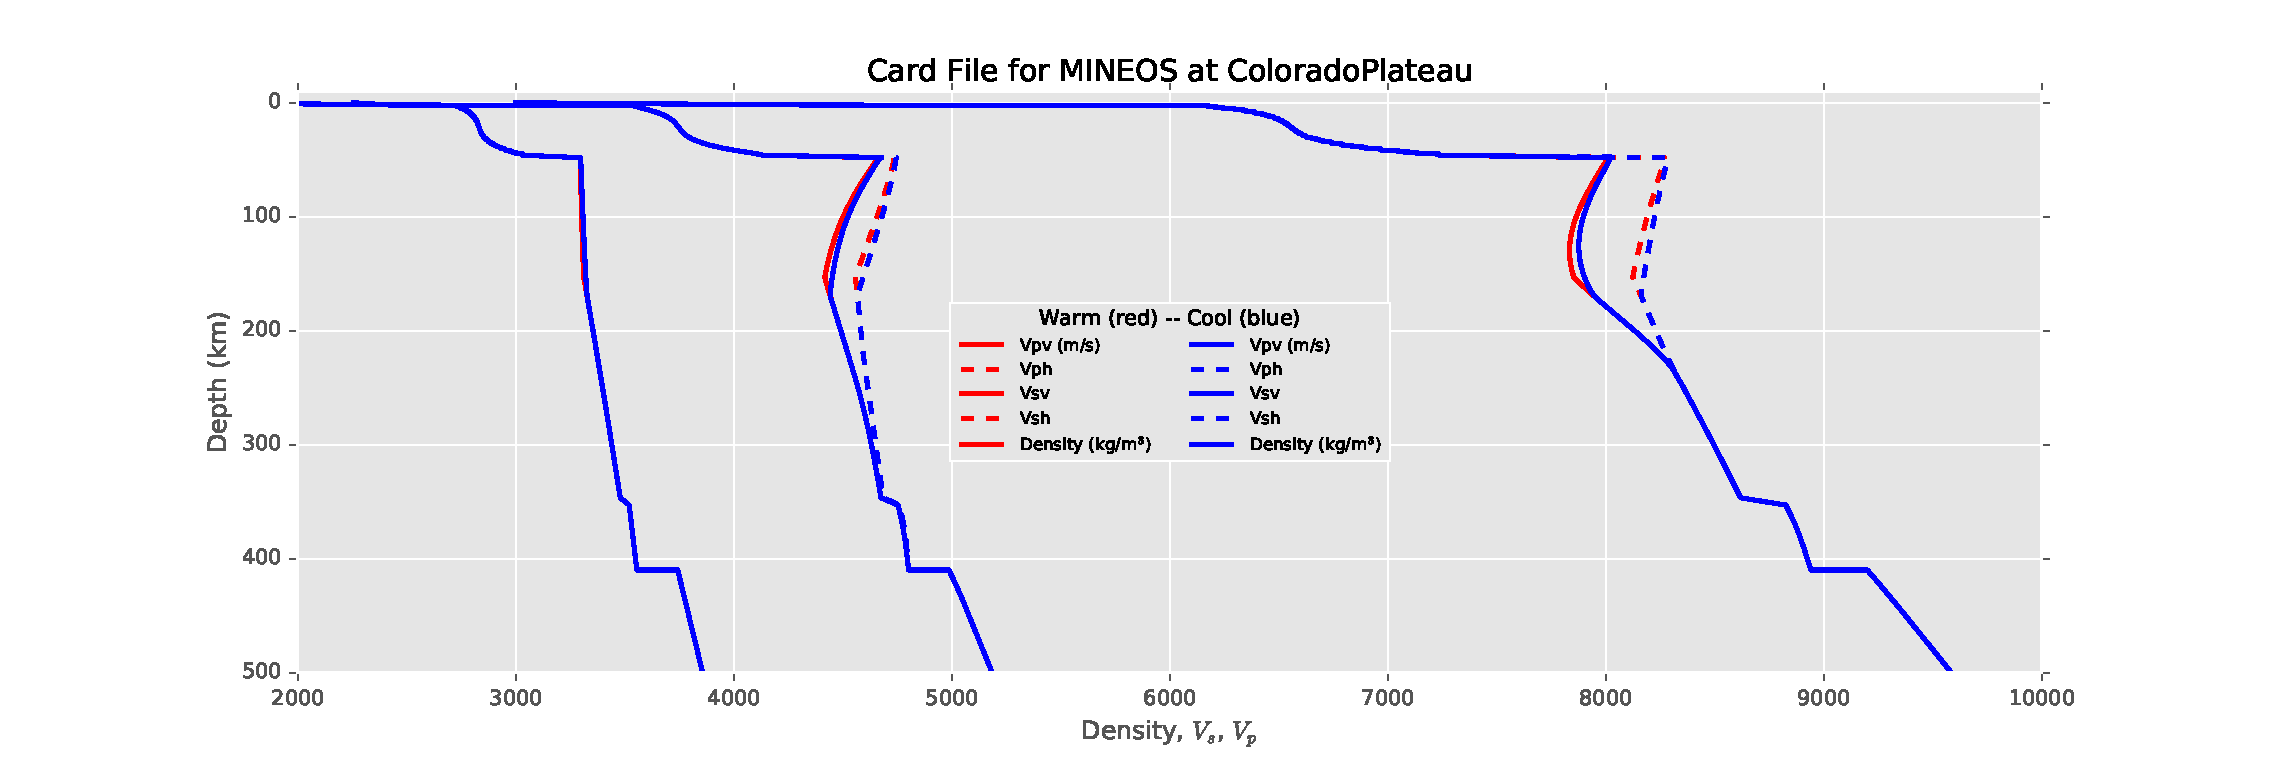
\includegraphics[width=1.0\textwidth]{img2/ColoradoPlateau_dunite_cardfile.eps} \\
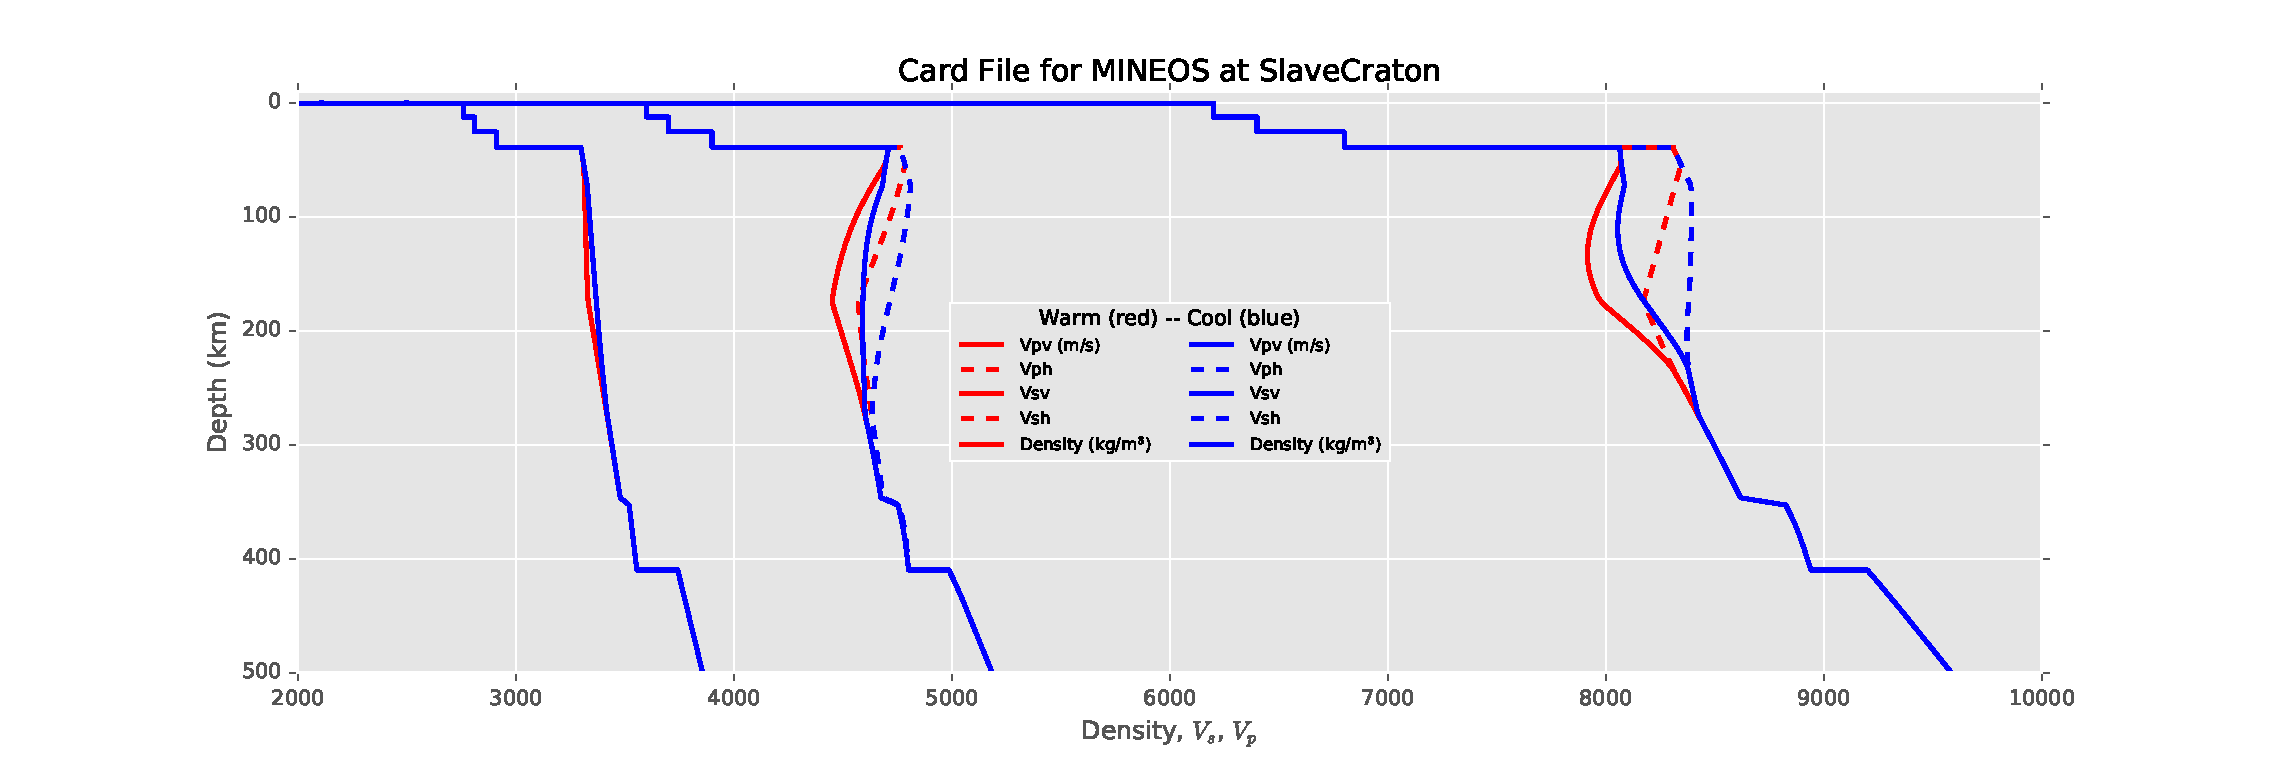
\includegraphics[width=1.0\textwidth]{img2/SlaveCraton_dunite_cardfile.eps} \\
\caption{Example material properties for a dunitic composition at the Colorado Plateau (upper) and Slave Craton (lower).}
\end{figure}

%\item Different PerpleX database files give different answers.  We have reason to believe Stixrude (2011) is the most reliable for anhydrous mantle calculations.

%\begin{figure}
%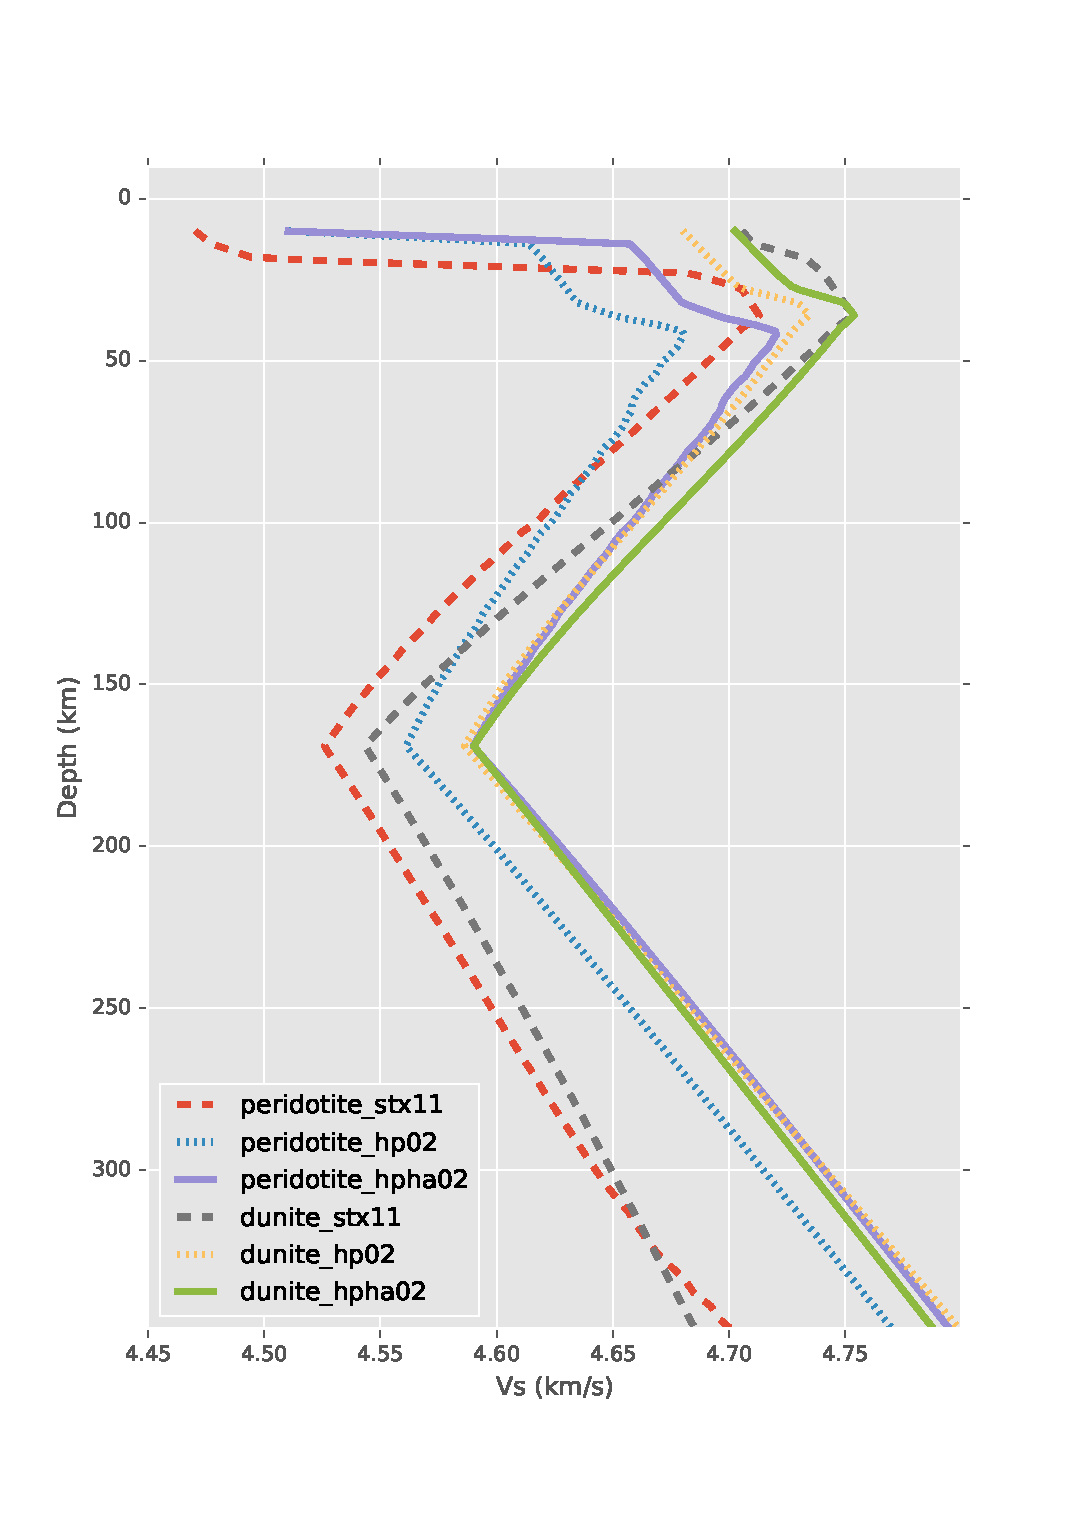
\includegraphics[width=0.3\textwidth]{img2/perplex_databases.eps}
%\caption{A comparison of databases.}
%\end{figure}


\end{itemize}

\end{block}

%----------------------------------------------------------------------------------------

\end{column} % End of column 2.2

\end{columns} % End of the split of column 2 - any content after this will now take up 2 columns width


\begin{columns}[t,totalwidth=\twocolwid] % Split up the two columns wide column again

\begin{column}{\onecolwid} % The first column within column 2 (column 2.1)

%----------------------------------------------------------------------------------------
%	OBSERVATIONS
%----------------------------------------------------------------------------------------

\begin{alertblock}{Comparison with Observations}

\begin{itemize}

\item We use mineos to estimate phase velocities assuming

\begin{itemize}

\item $V_{p}$, $V_{s}$ $\rightarrow$ $V_{pv}$, $V_{ph}$, $V_{sv}$, and $V_{sh}$ using the Voigt average and by taking scalings from the radially anisotropic reference model STW105.
\item crustal structure from Crust1.0 (Slave) or Shen and Ritzwoller (Colo. Plateau)
\item $Q_\mu$ from the geotherm predicted using Faul and Jackson (XXXX)

\end{itemize}

\begin{figure}
%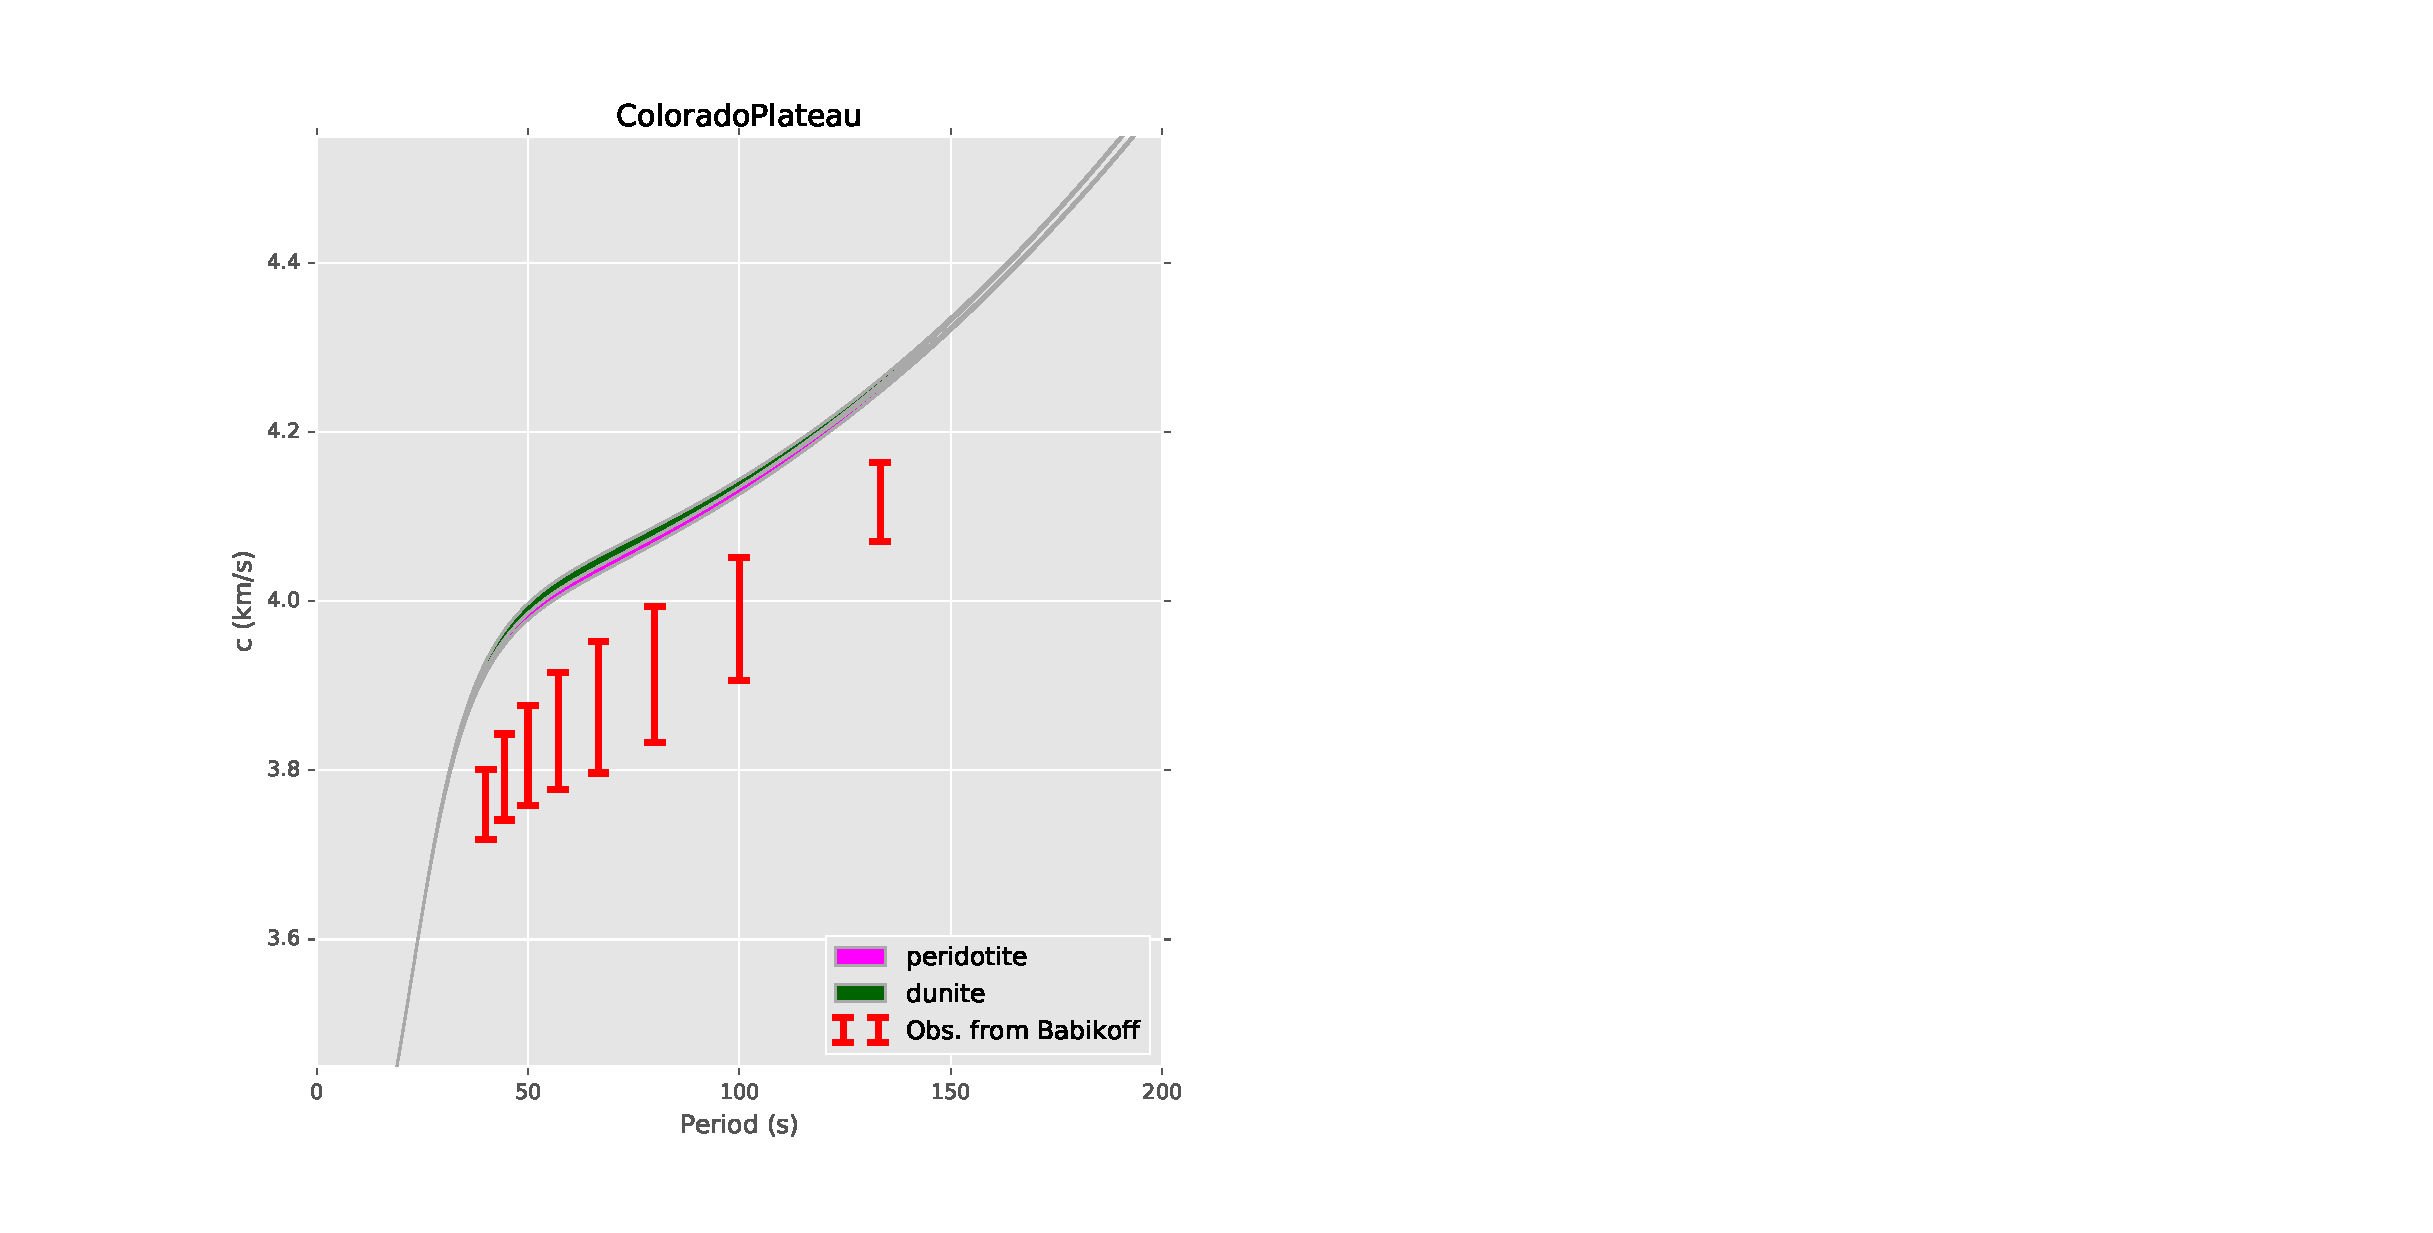
\includegraphics[width=0.3\textwidth]{img2/ColoradoPlateau_observations.eps}
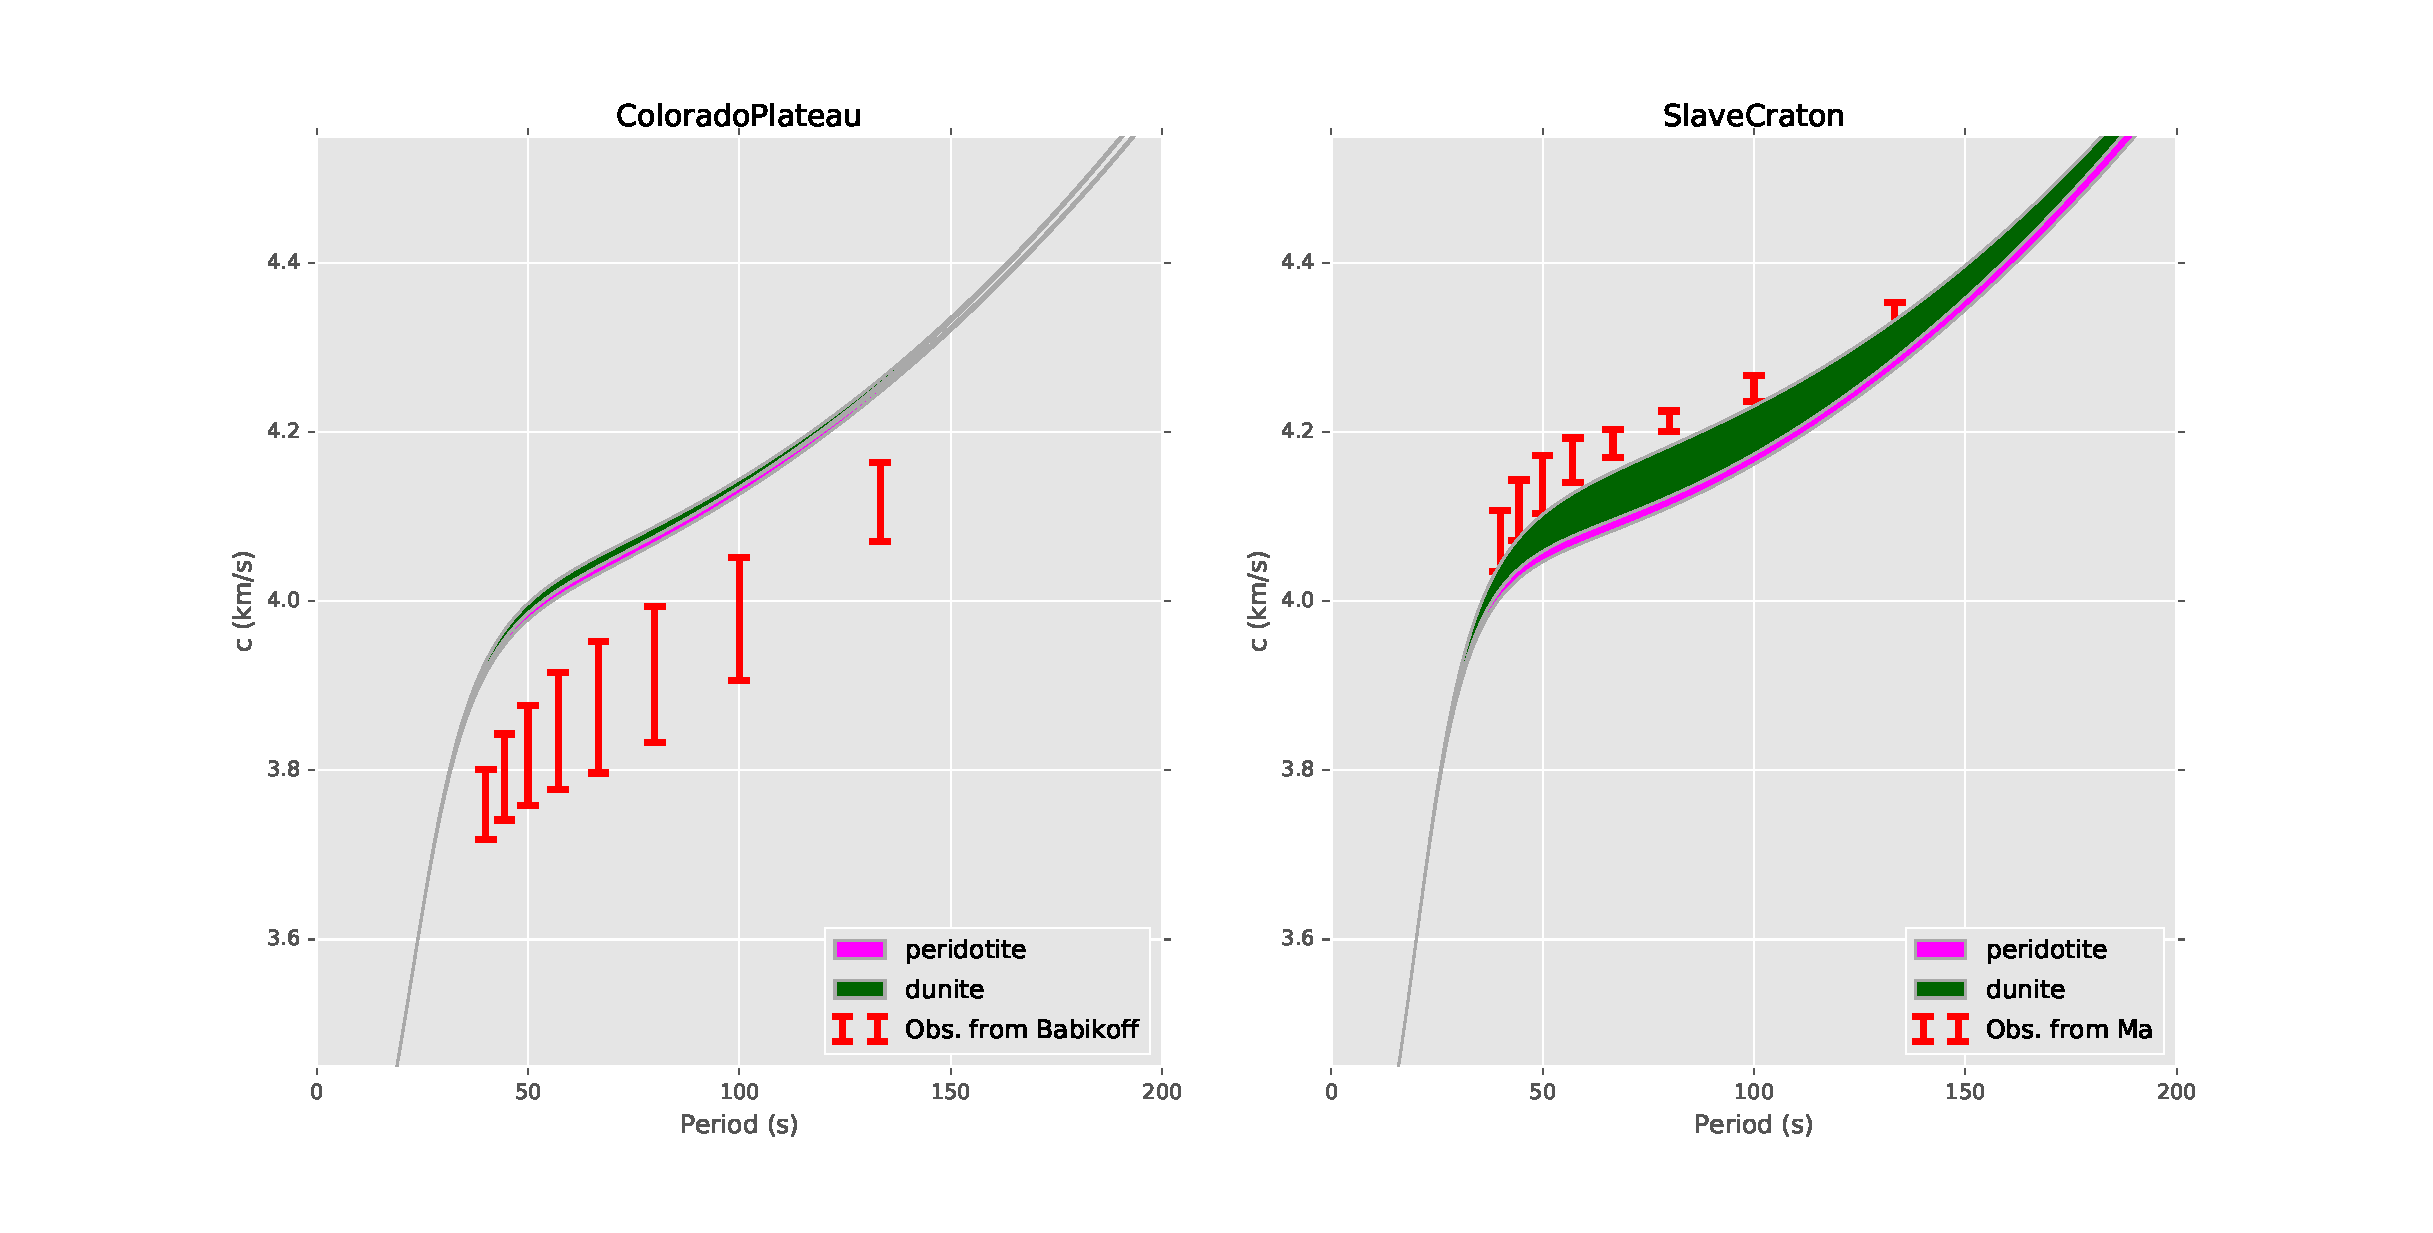
\includegraphics[width=0.8\textwidth]{img2/observations.eps}
\caption{Rayleigh phase predictions (colored shading) versus observation (red errorbars).}
\end{figure}

\end{itemize}

\end{alertblock}

%----------------------------------------------------------------------------------------

\end{column} % End of column 2.1

\begin{column}{\onecolwid} % The second column within column 2 (column 2.2)

%----------------------------------------------------------------------------------------
%	SS Precursors
%----------------------------------------------------------------------------------------

\begin{block}{SS Precursors}

\begin{figure}
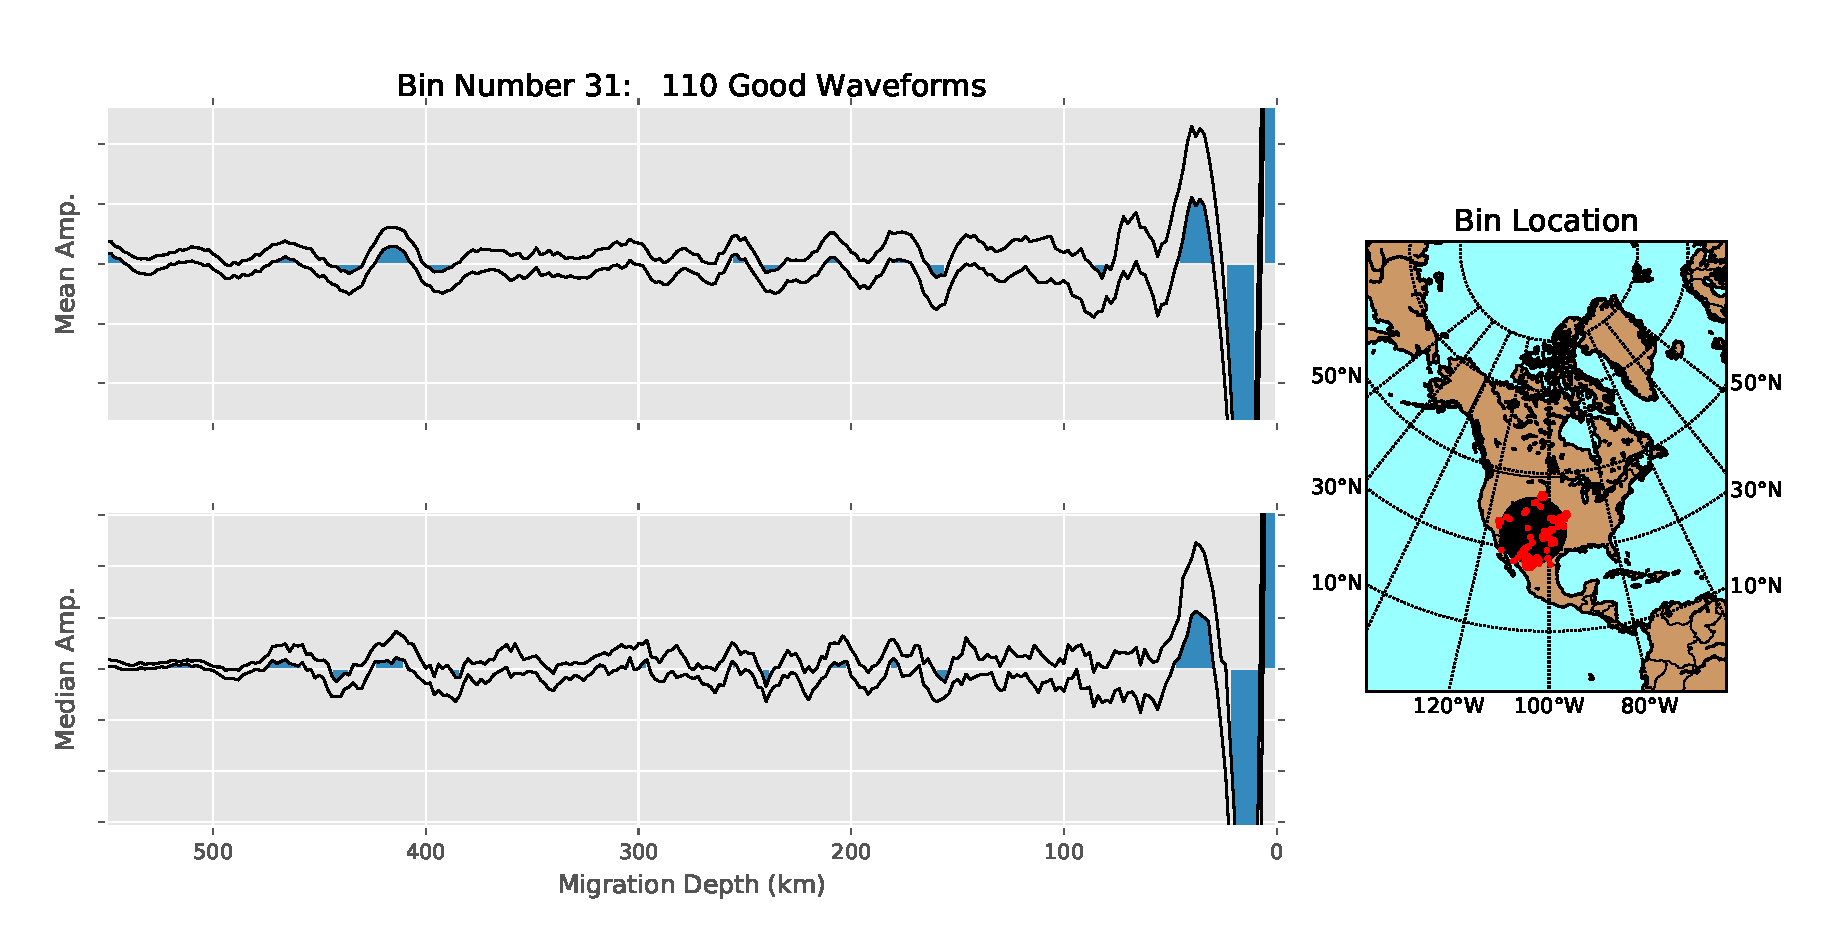
\includegraphics[width=0.8\textwidth]{img3/bin_31.eps} \\
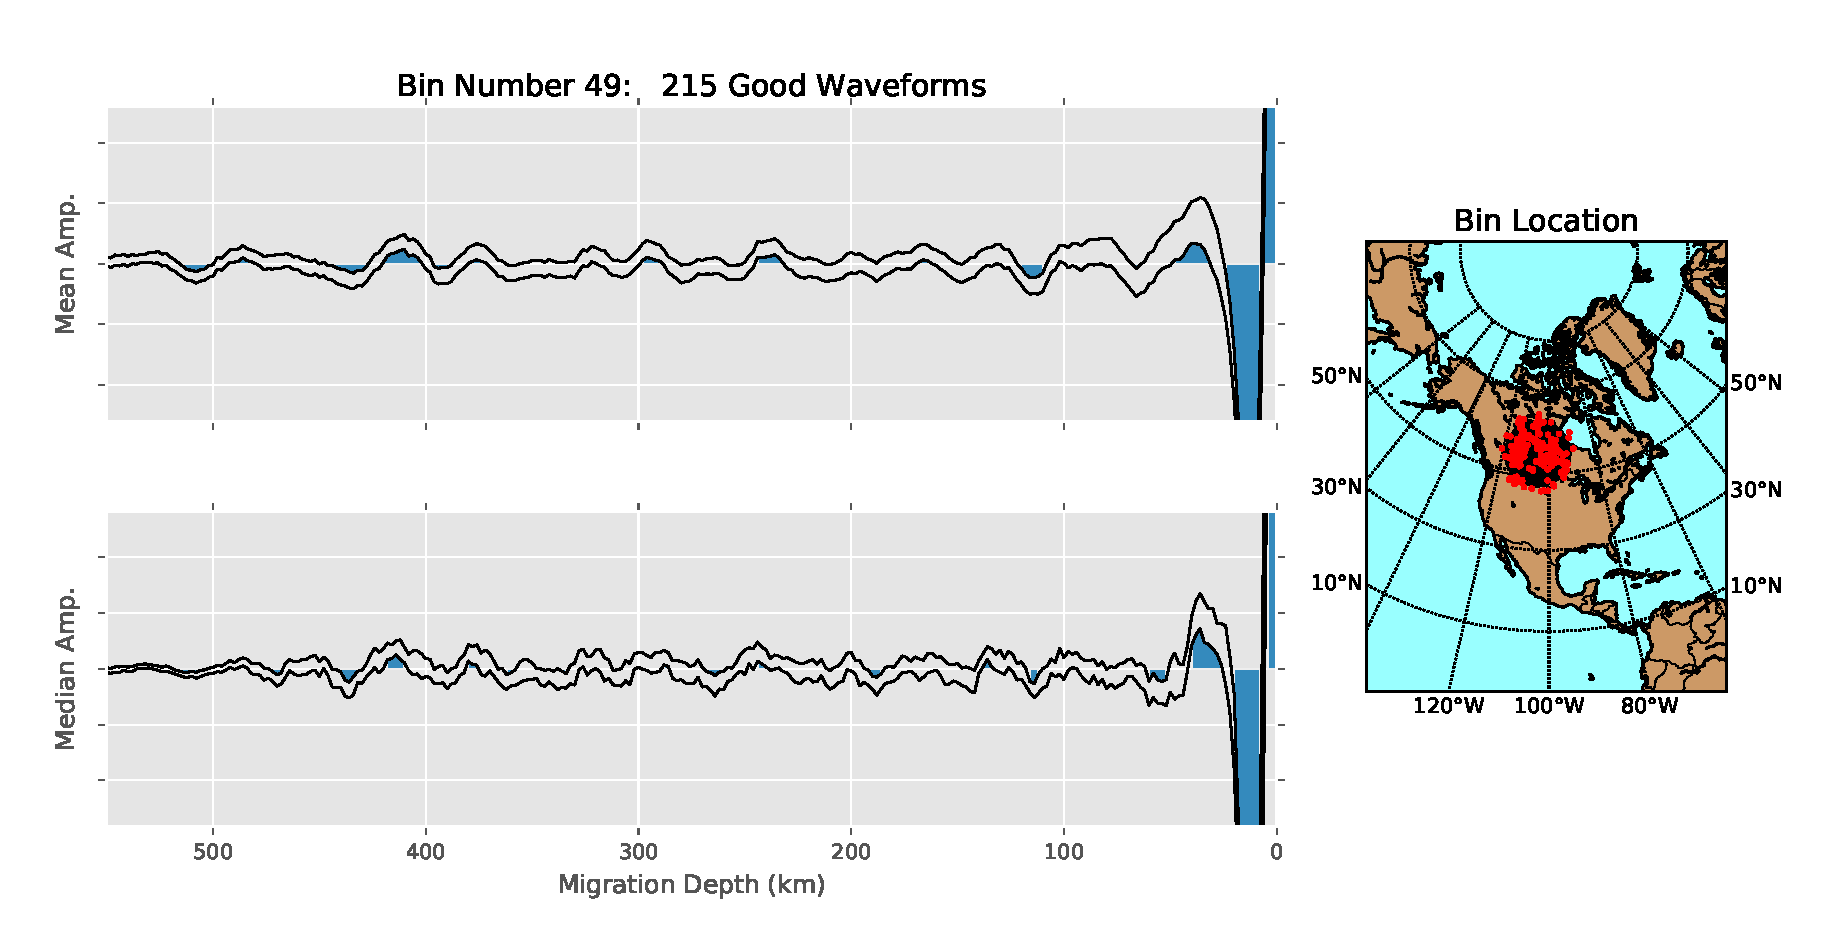
\includegraphics[width=0.8\textwidth]{img3/bin_49.eps}
\caption{SS precursor stacks for Colorado Plateau (upper) and Slave Craton (lower), with $1\sigma$ uncertainties.  The maps show individual bouncepoint locations (red dots). }
\end{figure}

\begin{itemize}

\item Traces are migrated through a reference velocity model, stacked in depth relative to peak SS, binned within 10 degree caps

\end{itemize}


\end{block}

%----------------------------------------------------------------------------------------

\end{column} % End of column 2.2

\end{columns} % End of the split of column 2

\end{column} % End of the second column

\begin{column}{\sepwid}\end{column} % Empty spacer column

\begin{column}{\onecolwid} % The third column

%----------------------------------------------------------------------------------------
%	Joint Inversions
%----------------------------------------------------------------------------------------

\begin{block}{Preliminary Joint Inversions}

\begin{itemize}

\item We use an iterative, linearized inversion technique to estimate a layer-cake model of shear velocities using constraints from (1) the stacked SS waveform and (2) from Rayleigh phase velocity observations.  Additional constraints:

	\begin{itemize}

	\item $d \ln V_{sv} = d \ln V_{sh} = 0.55 \ln V_{pv} = 0.55 d \ln V_{ph}$
	\item $d \ln \rho = 0$

	\end{itemize}

\item We have found it difficult to fit the large oscillations near SS, so these examples use synthetic SS precursor waveforms that approximate the phases observed in the stacks.

\end{itemize}

\begin{figure}

\includegraphics{img/placeholder.jpg}
\caption{Colorado Plateau Stack.}
\end{figure}

\begin{figure}

\includegraphics{img/placeholder.jpg}
\caption{Colorado Plateau Stack.}
\end{figure}


\end{block}

%----------------------------------------------------------------------------------------
%	REFERENCES
%----------------------------------------------------------------------------------------

\begin{block}{References}


\nocite{*} % Insert publications even if they are not cited in the poster
\tiny{\bibliographystyle{unsrt}
\bibliography{sample}\vspace{0.75in}}

\end{block}

%----------------------------------------------------------------------------------------
%	ACKNOWLEDGEMENTS
%----------------------------------------------------------------------------------------

%\setbeamercolor{block title}{fg=red,bg=white} % Change the block title color

\begin{block}{Acknowledgements}

\tiny{\rmfamily{For providing access and support for SPECFEM2D, we thank the Computational Infrastructure for Geodynamics (http://geodynamics.org) which is funded by the National Science Foundation under awards EAR-0949446 and EAR-1550901. This research was conducted using computational resources and services at the Center for Computation and Visualization, Brown University.
Funding for this research was provided by the NSF EarthScope Program  under award EAR-1614066.}} \\

\end{block}

\footnotetext{For full manuscript, contact nicholas\_mancinelli@brown.edu.}

%----------------------------------------------------------------------------------------
%	CONTACT INFORMATION
%----------------------------------------------------------------------------------------

%\setbeamercolor{block alerted title}{fg=black,bg=norange} % Change the alert block title colors
%\setbeamercolor{block alerted body}{fg=black,bg=white} % Change the alert block body colors

%\begin{alertblock}{Contact}
%\small{
%This work is currently in preparation for publication.  For a copy of the manuscript %please contact N.J. Mancinelli at
%\begin{itemize}
%\item \href{mailto:nicholas\_mancinelli@brown.edu}{nicholas\_mancinelli@brown.edu}.
%\end{itemize}
%}
%\end{alertblock}

%\begin{center}
%\begin{tabular}{ccc}
%
\includegraphics[width=0.4\linewidth]{logo.png} & \hfill & %
\includegraphics[width=0.4\linewidth]{logo.png}
%\end{tabular}
%\end{center}

%----------------------------------------------------------------------------------------

\end{column} % End of the third column

\end{columns} % End of all the columns in the poster

\end{frame} % End of the enclosing frame

\end{document}
